%package list
\documentclass{article}
\usepackage[top=3cm, bottom=3cm, outer=3cm, inner=3cm]{geometry}
\usepackage{multicol}
\usepackage{graphicx}
\usepackage{url}
%\usepackage{cite}
\usepackage{hyperref}
\usepackage{array}
%\usepackage{multicol}
\newcolumntype{x}[1]{>{\centering\arraybackslash\hspace{0pt}}p{#1}}
\usepackage{natbib}
\usepackage{pdfpages}
\usepackage{multirow}    
\usepackage[normalem]{ulem}
\useunder{\uline}{\ul}{}
\usepackage{svg}
\usepackage{xcolor}
\usepackage{listings}
\lstdefinestyle{ascii-tree}{
    literate={├}{|}1 {─}{--}1 {└}{+}1 
  }
\lstset{basicstyle=\ttfamily,
  showstringspaces=false,
  commentstyle=\color{red},
  keywordstyle=\color{blue}
}
%\usepackage{booktabs}
\usepackage{caption}
\usepackage{subcaption}
\usepackage{float}
\usepackage{array}

\usepackage{enumitem}


\newcolumntype{M}[1]{>{\centering\arraybackslash}m{#1}}
\newcolumntype{N}{@{}m{0pt}@{}}


%%%%%%%%%%%%%%%%%%%%%%%%%%%%%%%%%%%%%%%%%%%%%%%%%%%%%%%%%%%%%%%%%%%%%%%%%%%%
%%%%%%%%%%%%%%%%%%%%%%%%%%%%%%%%%%%%%%%%%%%%%%%%%%%%%%%%%%%%%%%%%%%%%%%%%%%%
\newcommand{\itemEmail}{vmaldonadov@unsa.edu.pe}
\newcommand{\itemStudent}{Victor Gonzalo Maldonado Vilca}
\newcommand{\itemCourse}{Programación Web 2}
\newcommand{\itemCourseCode}{1702122}
\newcommand{\itemSemester}{III}
\newcommand{\itemUniversity}{Universidad Nacional de San Agustín de Arequipa}
\newcommand{\itemFaculty}{Facultad de Ingeniería de Producción y Servicios}
\newcommand{\itemDepartment}{Departamento Académico de Ingeniería de Sistemas e Informática}
\newcommand{\itemSchool}{Escuela Profesional de Ingeniería de Sistemas}
\newcommand{\itemAcademic}{2024 - A}
\newcommand{\itemInput}{Del 10 de mayo de 2024}
\newcommand{\itemOutput}{Al 26 de mayo de 2024}
\newcommand{\itemPracticeNumber}{04}
\newcommand{\itemTheme}{Práctica SQLite}
%%%%%%%%%%%%%%%%%%%%%%%%%%%%%%%%%%%%%%%%%%%%%%%%%%%%%%%%%%%%%%%%%%%%%%%%%%%%
%%%%%%%%%%%%%%%%%%%%%%%%%%%%%%%%%%%%%%%%%%%%%%%%%%%%%%%%%%%%%%%%%%%%%%%%%%%%

\usepackage[english,spanish]{babel}
\usepackage[utf8]{inputenc}
\AtBeginDocument{\selectlanguage{spanish}}
\renewcommand{\figurename}{Figura}
\renewcommand{\refname}{Referencias}
\renewcommand{\tablename}{Tabla} %esto no funciona cuando se usa babel
\AtBeginDocument{%
	\renewcommand\tablename{Tabla}
}

\usepackage{fancyhdr}
\pagestyle{fancy}
\fancyhf{}
\setlength{\headheight}{30pt}
\renewcommand{\headrulewidth}{1pt}
\renewcommand{\footrulewidth}{1pt}
\fancyhead[L]{\raisebox{-0.2\height}{
\includegraphics[width=3cm]{img/logo_episunsa.png}}}
\fancyhead[C]{\fontsize{7}{7}\selectfont	\itemUniversity \\ \itemFaculty \\ \itemDepartment \\ \itemSchool \\ \textbf{\itemCourse}}
\fancyhead[R]{\raisebox{-0.2\height}{
\includegraphics[width=1.2cm]{img/logo_abet}}}
\fancyfoot[L]{Victor M.}
\fancyfoot[C]{\itemCourse}
\fancyfoot[R]{Página \thepage}

% para el codigo fuente
\usepackage{listings}
\usepackage{color, colortbl}
\definecolor{dkgreen}{rgb}{0,0.6,0}
\definecolor{gray}{rgb}{0.5,0.5,0.5}
\definecolor{mauve}{rgb}{0.58,0,0.82}
\definecolor{codebackground}{rgb}{0.95, 0.95, 0.92}
\definecolor{tablebackground}{rgb}{0.8, 0, 0}

\lstset{frame=tb,
	language=bash,
	aboveskip=3mm,
	belowskip=3mm,
	showstringspaces=false,
	columns=flexible,
	basicstyle={\small\ttfamily},
	numbers=none,
	numberstyle=\tiny\color{gray},
	keywordstyle=\color{blue},
	commentstyle=\color{dkgreen},
	stringstyle=\color{mauve},
	breaklines=true,
	breakatwhitespace=true,
	tabsize=3,
	backgroundcolor= \color{codebackground},
}
\lstdefinelanguage{JavaScript}{
  keywords={typeof, new, true, false, catch, function, return, null, catch, switch, var, if, in, while, do, else, case, break},
  keywordstyle=\color{blue}\bfseries,
  ndkeywords={class, export, boolean, throw, implements, import, this},
  ndkeywordstyle=\color{darkgray}\bfseries,
  identifierstyle=\color{black},
  sensitive=false,
  comment=[l]{//},
  morecomment=[s]{/*}{*/},
  commentstyle=\color{purple}\ttfamily,
  stringstyle=\color{red}\ttfamily,
  morestring=[b]',
  morestring=[b]"
}
\lstset{
  language=JavaScript,
  basicstyle=\ttfamily, 
  keywordstyle=\color{blue}, 
  commentstyle=\color{green},
  numbers=left, 
  numberstyle=\tiny\color{gray},
  breaklines=true 
}

\lstdefinelanguage{CSS}{
  keywords={color, background-color, border, ...}, 
  keywordstyle=\color{blue},
  comment=[l]{//}, 
  morecomment=[s]{/*}{*/}, 
  commentstyle=\color{green},
}

\begin{document}
	
	\vspace*{10px}
	
	\begin{center}	
		\fontsize{17}{17} \textbf{Informe de SQLite}
	\end{center}
	\centerline{\textbf{\Large Tema: \itemTheme}}
	%\vspace*{0.5cm}	

	\begin{flushright}
		\begin{tabular}{|M{2.5cm}|N|}
			\hline 
			\rowcolor{tablebackground}
			\color{white} \textbf{Nota}  \\
			\hline 
			     \\[30pt]
			\hline 			
		\end{tabular}
	\end{flushright}	

	\begin{table}[H]
		\begin{tabular}{|x{4.7cm}|x{4.8cm}|x{4.8cm}|}
			\hline 
			\rowcolor{tablebackground}
			\color{white} \textbf{Estudiante} & \color{white}\textbf{Escuela}  & \color{white}\textbf{Asignatura}   \\
			\hline 
			{\itemStudent \par \itemEmail} & \itemSchool & {\itemCourse \par Semestre: \itemSemester \par Código: \itemCourseCode}     \\
			\hline 			
		\end{tabular}
	\end{table}		
	
	\begin{table}[H]
		\begin{tabular}{|x{4.7cm}|x{4.8cm}|x{4.8cm}|}
			\hline 
			\rowcolor{tablebackground}
			\color{white}\textbf{Tarea} & \color{white}\textbf{Tema}  & \color{white}\textbf{Duración}   \\
			\hline 
			\itemPracticeNumber & \itemTheme & 2 horas   \\
			\hline 
		\end{tabular}
	\end{table}
	
	\begin{table}[H]
		\begin{tabular}{|x{4.7cm}|x{4.8cm}|x{4.8cm}|}
			\hline 
			\rowcolor{tablebackground}
			\color{white}\textbf{Semestre académico} & \color{white}\textbf{Fecha de inicio}  & \color{white}\textbf{Fecha de entrega}   \\
			\hline 
			\itemAcademic & \itemInput &  \itemOutput  \\
			\hline 
		\end{tabular}
	\end{table}
%%%%%%%%%%%%%%%%%%%%

  \section{Introducción}
  \subsection{Node.js}
    Es una plataforma de tiempo de ejecución de JavaScript que permite ejecutar código JavaScript en el servidor. 
    Con Node.js, podemos crear servidores web eficientes y escalables. Es especialmente útil en el desarrollo de 
    aplicaciones web en tiempo real y aplicaciones de una sola página que requieren una comunicación constante entre 
    el cliente y el servidor.
  \subsection{Ajax}
    Es una tecnología que permite actualizar partes específicas de una página web sin necesidad de recargarla por completo. 
    Con AJAX, las solicitudes al servidor se realizan de forma asíncrona, lo que significa que el usuario puede interactuar con 
    la página sin interrupciones. Esto mejora significativamente la experiencia del usuario al proporcionar respuestas rápidas y dinámicas.
  \subsection{Json}
    Es un formato ligero y legible para el intercambio de datos entre el cliente y el servidor. Es fácil de entender tanto 
    para los humanos como para las máquinas, lo que lo hace ideal para la comunicación en aplicaciones web. JSON se utiliza 
    comúnmente para enviar datos entre el cliente y el servidor, ya sea en respuesta a solicitudes AJAX o para almacenar datos 
    en bases de datos.
  \newpage
  \subsection{SQL}
    Es un lenguaje de programación utilizado para administrar bases de datos relacionales. Con SQL, podemos crear, leer, 
    actualizar y eliminar datos en una base de datos de manera eficiente. Es fundamental en el desarrollo web para almacenar 
    y manipular datos de manera estructurada.
  \subsection{mySQL}
    Es un sistema de gestión de bases de datos relacionales (RDBMS) ampliamente utilizado y de código abierto. 
    Destaca por su rendimiento, confiabilidad y facilidad de uso, siendo una opción popular para una variedad de aplicaciones, 
    desde pequeños sitios web hasta grandes sistemas empresariales.
  
%%%%%%%%%%%%%%%%%%%%

  \section{Objetivos}
  \begin{itemize}
    \item Crear una aplicación web que utilice SQLite para poder manipular información de películas.
    \item Implementar la comunicación entre el cliente y el servidor utilizando AJAX y JSON.
  \end{itemize}

%%%%%%%%%%%%%%%%%%%%
 
	\section{Tarea}
  \begin{itemize}
    \item Realice un ejemplo de sqlite libre, con la base de datos imdb.db, tendrá que usar ajax y json 
      para la comunicación entre cliente y servidor; así como git para sus versiones. No es necesario que 
      entregue un programa funcionando, pero si es importante que muestre los errores encontrados.
  \end{itemize}
  
%%%%%%%%%%%%%%%%%%%% 
 
  \section{Entregables}
  \begin{itemize}
    \item Informe del proyecto
    \item Repositorio en gitHub
    \item Link del vídeo Explicativo
  \end{itemize}
  
%%%%%%%%%%%%%%%%%%%%    
		
	\section{Equipos, materiales y temas utilizados}
  \begin{itemize}
    \item Node.js
    \item JavaScript
    \item Ajax
    \item Json
    \item Xampp
    \item SQL
    \item mySQL
  \end{itemize}
 
%%%%%%%%%%%%%%%%%%%%

  \section{URL de Repositorio Github}
  \begin{itemize}
    \item URL: Repositorio SQLite en GitHub
    \item \url{https://github.com/Victor-Gonzalo-Maldonado-Vilca/SQLite.git}
  \end{itemize}
  \newpage
  
%%%%%%%%%%%%%%%%%%%%

	\section{Link de Video}
  \begin{itemize}
    \item Link del vídeo explicativo
    \item \url{https://www.youtube.com/watch?v=GqJOymFuurA}
  \end{itemize}

%%%%%%%%%%%%%%%%%%%%

  \section{Metodología}

%%%%%%%%%%%%

  \subsection{Creación del entorno de trabajo}
  \textit{(Tener instalado Node.js)}
  
%%%%%%
  
  \subsubsection{Creación de carpetas}
  \begin{itemize}
    \item Directorio Actual \textit{(Nos encontraremos en la siguiente ruta)}
    \begin{lstlisting}[language=,caption=Directorio Actual]
      D:\UNSA\PW2\Teoria\SQLite\src
    \end{lstlisting}
    \item Creamos carpeta de Trabajo
    \begin{lstlisting}[language=,caption=Carpeta de Trabajo]
      mkdir Programa && cd Programa
    \end{lstlisting}
  \end{itemize}

%%%%%%

  \subsubsection{Instalar modulos necesarios}
  \textit{(Recordar: Agregar la ruta de instalación de Node.js y npm a las variables de entorno)}
  \begin{itemize}
    \item \textbf{Instalar Modulo Express:}
    \begin{lstlisting}[language=,caption=Install Express]
      npm install express
    \end{lstlisting}
    \item \textbf{Instalar Modulo mySQL:}
    \begin{lstlisting}[language=,caption=Install mySQL]
      npm install mysql
    \end{lstlisting}
  \end{itemize}

%%%%%%%%%%%%

  \subsection{Uso de Xampp}
  \textit{(Tener instalado xampp)}
  
%%%%%%

  \subsubsection{Descripción}
    Es un paquete de software que incluye Apache, MySQL, PHP y Perl. Permite crear fácilmente un entorno 
    de desarrollo web local en sistemas Windows, Linux y macOS. Es ampliamente utilizado por desarrolladores 
    web para comenzar a desarrollar y probar aplicaciones sin tener que configurar cada componente por separado.
  \newpage
  
%%%%%%

  \subsubsection{Activar puertos mysql y apache de xampp}
  \begin{figure}[H]
    \centering
    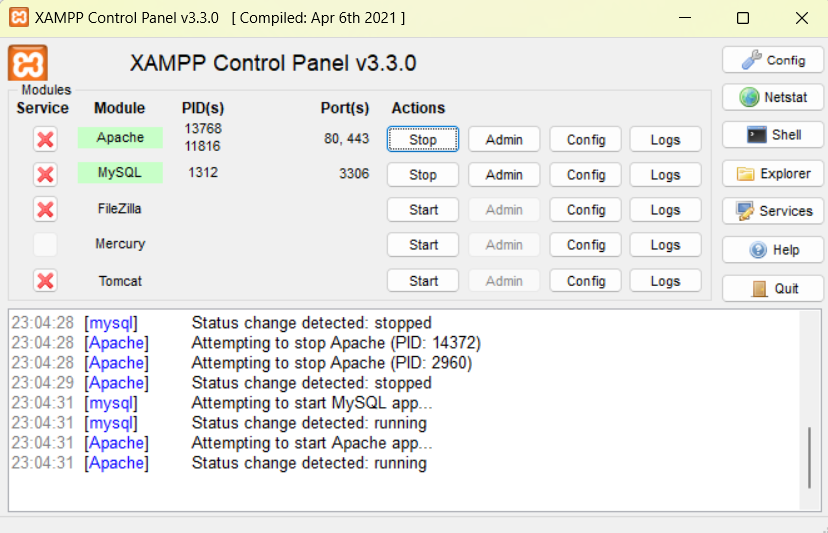
\includegraphics[width=1\textwidth, keepaspectratio]{img/puertos.png}
    \caption{Activación de puertos}
  \end{figure}
  
%%%%%%

  \subsubsection{Uso del archivo imdb.db}
  \begin{figure}[H]
    \centering
    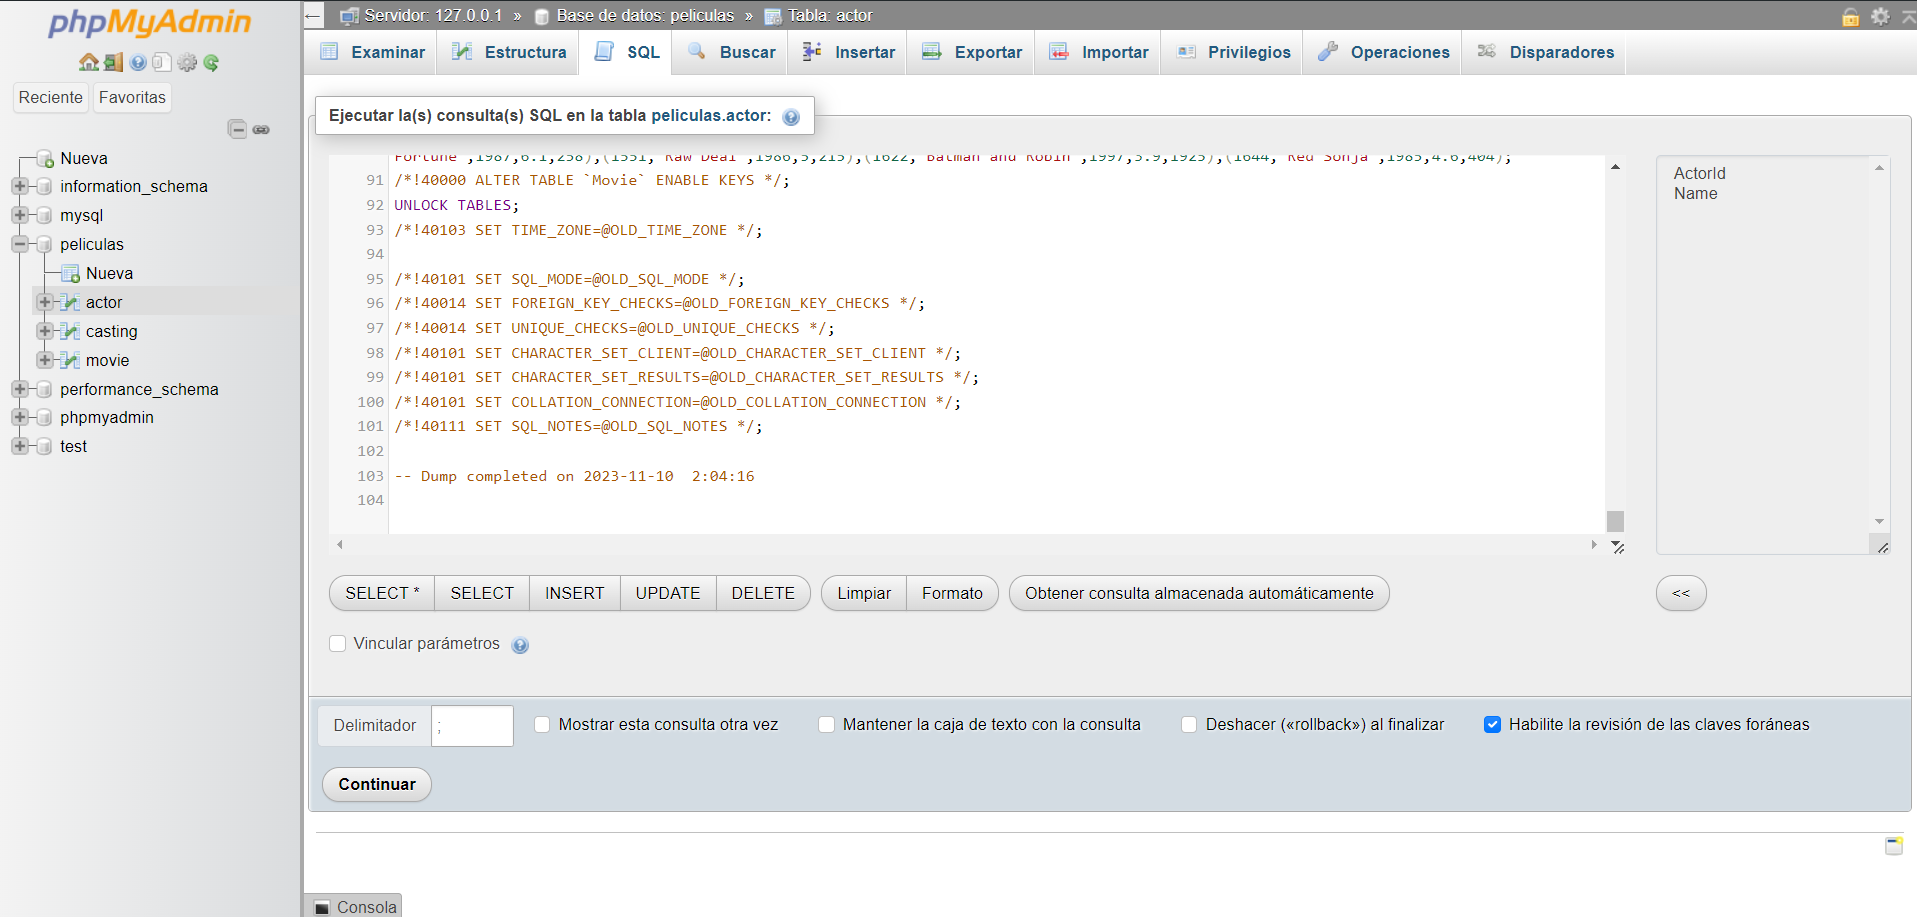
\includegraphics[width=1\textwidth, keepaspectratio]{img/crearTablas.png}
    \caption{Uso de imdb.db}
  \end{figure}
  \newpage

%%%%%%%%%%%%%%%%%%%%

  \section{Desarrollo del trabajo}
  
%%%%%%%%%%%%

  \subsection{Archivo index.js \textit{(Parte - Servidor)}}
  
%%%%%%

  \subsubsection{Fragmentos del Código}
  \begin{itemize}
    \item En esta parte se importa los módulos path, express, body-parser y mysql, y luego crea una instancia de la 
      aplicación Express. Estos módulos son utilizados para manejar rutas de archivos, configurar el servidor web, 
      analizar datos enviados desde formularios HTML, y conectar y comunicarse con una base de datos MySQL.
    \begin{lstlisting}[language=JavaScript,caption=Importación]
      const path = require('path');
      const express = require('express');
      const bp = require('body-parser');
      const mysql = require('mysql')
      const app = express();
    \end{lstlisting}
    \item Esta sección del código configura el servidor Express para servir archivos estáticos desde el directorio 'pub'
      , analizar datos JSON y analizar datos de formularios HTML.
    \begin{lstlisting}[language=JavaScript,caption=Configuración,firstnumber=7]
      app.use(express.static('pub'));
      app.use(bp.json());
      app.use(bp.urlencoded({ extended: true }));
    \end{lstlisting}
    \item Este fragmento de código inicia el servidor Express en el puerto 3000 y muestra un mensaje en la consola 
      indicando que el servidor está escuchando en la dirección http://localhost:3000.
    \begin{lstlisting}[language=JavaScript,caption=Servidor Inicial,firstnumber=12]
      app.listen(3000, () => {
        console.log("Escuchando en: http://localhost:3000")
      });
    \end{lstlisting}
    \item Este bloque de código establece una conexión a una base de datos MySQL en el servidor local. 
      Se especifican los detalles de la conexión, incluyendo el host, el puerto, el nombre de usuario, la contraseña 
      y el nombre de la base de datos a la que se desea conectar. En este caso, se está intentando conectar a una base de 
      datos llamada 'peliculas' con el usuario 'Victor' y la contraseña proporcionada.
    \begin{lstlisting}[language=JavaScript,caption=conexion mySQL,firstnumber=20]
      const conexion = mysql.createConnection({
        host: 'localhost',
        port: 3306,
        user: 'Victor',
        password: 'maldonado100204.',
        database: 'peliculas'
      });
    \end{lstlisting}
    \item Este bloque de código establece una conexión a una base de datos MySQL y define una ruta en la aplicación 
      Express para manejar solicitudes POST en '/basedata'. \newline Cuando se recibe una solicitud POST en esa ruta, se extrae 
      un dato del cuerpo de la solicitud y se realiza una consulta SQL a la base de datos utilizando ese dato como parámetro. 
      Si la consulta es exitosa, se devuelve el resultado al cliente en formato JSON. Si hay un error durante la conexión o la 
      consulta, se devuelve un mensaje de error al cliente.
    \begin{lstlisting}[language=JavaScript,caption=consulta mySQL,firstnumber=28]
      conexion.connect((err) => {
        if (err) {
          console.error('Error de conexion mysql ', err);
          return;
        } else {
          console.log('Conexion Establecida mysql')
        }
        
        app.post('/basedata',(request, response) => {
          const fecha = request.body.year;
          console.log(fecha);
          //consulta sql
          conexion.query('SELECT * FROM movie WHERE Year = ?',[fecha],(err,filas) => {
            if (err) {
              console.error('Error en la consulta')
              response.status(500).json({error: 'Error en la consulta'});
            } else {
              //Respuesta del servidor
              console.log('Consulta realizada')
              response.json(filas);
            }
          });
        });
      });
    \end{lstlisting}
  \end{itemize}
  
%%%%%%%%%%%%

  \subsection{Archivo index.html}
  
%%%%%%

  \subsubsection{Fragmentos del Código}
  \begin{itemize}
    \item Este fragmento de código HTML define la estructura básica de una página web con el título "SQLite" y metadatos 
      como el autor y la descripción. También enlaza un archivo CSS externo llamado "estilos.css" para aplicar estilos a la página.
    \begin{lstlisting}[language=HTML,caption=Head,,firstnumber=4]
      <title>SQLite</title>
      <meta charset="utf-8"/>
      <meta name="author" content="Victor Gonzalo Maldonado Vilca"/>
      <meta name="description" content="Ejemplo Libre SQLite"/>
      <link rel="stylesheet" href="estilos.css"/>
    \end{lstlisting}
    \newpage
    \item Este fragmento de código HTML crea una página web que muestra un título Tabla de Películas seguido de un 
      formulario para ingresar un año. El formulario incluye un campo de entrada de tipo número con restricciones de 
      rango para el año (de 1900 a 2024) y un botón de envío etiquetado como Generar. Cuando el formulario se envía, se 
      espera que se genere una tabla de películas relacionadas con el año ingresado. El resultado de la tabla se mostrará 
      en un contenedor con el id table.
    \begin{lstlisting}[language=HTML,caption=Body,firstnumber=12]
      <h1>Tabla de Peliculas</h1>
      <form id="formulario">
        <label for="year">Ingrese Year:</label>
        <input type="number" placeholder="Year superior a 1899 e inferior 2025" id="year" name="year" min="1900" max="2024"/>
        <input type="submit" value="Generar" id="submit"/>
      </form>
      <div id="table"></div>
    \end{lstlisting}
    \item Esta etiqueta script enlaza el archivo JavaScript programa.js con la página HTML actual. Esto permite 
      que el navegador cargue y ejecute el código JavaScript contenido en el archivo programa.js cuando se renderiza la página web.
    \begin{lstlisting}[language=HTML,caption=Script,firstnumber=20]
      <script src="programa.js"></script>
    \end{lstlisting}
  \end{itemize}
  
%%%%%%%%%%%%

  \subsection{Archivo programa.js \textit{(Se creo directorio 'pub' \protect\texttt{=>} Parte - Cliente)}}
  
%%%%%%

  \subsubsection{Fragmentos del Código}
  \begin{itemize}
    \item  Esta función recibe un parámetro fecha que representa el año de la película a buscar. 
      Luego, realiza una solicitud POST al servidor para obtener datos de películas relacionadas con ese año. 
      Una vez que recibe la respuesta del servidor, procesa los datos y los muestra en una tabla en la página HTML.
    \begin{lstlisting}[language=JavaScript,caption=function movies()]
      function movies(fecha){
        const url = 'http://localhost:3000/basedata';
        const data = {
          year: parseInt(fecha)
        }
        console.log(data);
        //Enviando datos al servidor, uso de json
        const request = {
          method: 'POST',
          headers: {
            'Content-Type': 'application/json',
          },
          body: JSON.stringify(data),
        }
        
        fetch(url, request)
          .then(response => response.json())
          .then(datos => {
            console.log(datos);
            const contenedorTabla = document.querySelector('#table');
            contenedorTabla.innerHTML = '';
            //Verificando que los datos extraidos no esten vacios
            if (datos.length > 0) {
              
              const tabla = document.createElement('table');
              tabla.classList = 'tablePeliculas';
              const encabezado = tabla.createTHead();
              const filaE = tabla.insertRow();
              
              //Agregar el encabezado, extrayendolo de la base de datos
              for (const key in datos[0]){
                if(key != 'id' && key != 'Year'){
                  const th = document.createElement('th');
                  th.textContent = key.toUpperCase();
                  filaE.appendChild(th);
                }
              }
              
              //Insertar filas donde se encontraran los datos correspondientes
              const cuerpoTabla = tabla.createTBody();
              datos.forEach(dato => {
                const fila = cuerpoTabla.insertRow();
                for (const key in dato){
                  if(key != 'id' && key != 'Year'){
                    const td = fila.insertCell();
                    td.textContent = dato[key];
                  }
                }
              })
              contenedorTabla.appendChild(tabla);
            } else {
              //Caso contrario se genera un parrafo con un texto correspondiente
              const texto = document.createElement('p');
              texto.id = 'text';
              texto.textContent = 'No hay Peliculas que mostrar';
              contenedorTabla.appendChild(texto);
            }
          })
      }
    \end{lstlisting}
    \item Este bloque de código se ejecuta cuando se carga completamente la página. Busca el elemento HTML 
      correspondiente al campo de entrada de year y configura un evento para el formulario. 
      Cuando se envía el formulario, se llama a la función movies(fecha.value) para obtener y mostrar las 
      películas relacionadas con el año ingresado.
    \begin{lstlisting}[language=HTML,caption=Evento,firstnumber=62]
      document.addEventListener('DOMContentLoaded', function(){
        //Extraer parametro del formulario
        const fecha = document.querySelector(#year);
        //Realizar ciertas funciones al presionar el boton del formulario
        document.querySelector('#formulario').onsubmit = (event) => {
          //Evita que se cargue nuevamente la pagina
          event.preventDefault();
          //llamada al metodo movies()
          movies(fecha.value);
          return false;
        }
      });
    \end{lstlisting}
  \end{itemize}

%%%%%%%%%%%%

  \subsection{Estilos \textit{(En el directorio 'pub')}}
  \begin{itemize}
    \item Estos estilos CSS definen el formato básico para una página web que incluye una tabla de películas 
      y un formulario para ingresar el año de las películas a visualizar. Incluyen ajustes de alineación, bordes 
      y colores para garantizar una apariencia consistente y agradable en la interfaz de usuario.
    \begin{lstlisting}[language=CSS,caption=Estilos]
      .tablePeliculas{
        text-align: center;
        border-collapse: collapse;
        margin-top: 10px;
      }

      .tablePeliculas td, .tablePeliculas th{
        border: 1px solid black;
      }

      h1 {
        color: #700000;
      }

      label {
        color: #700000;
      }

      #year {
        border-radius: 10px;
        border: 1px solid black;
        padding-left: 10px;
        width: 225px;
      }

      #submit {
        color: white;
        border: 1px solid #640000;
        background: #7e1919;
        border-radius: 10px;
      }

      #submit:hover {
        border: 1px solid #7e1919;
        background: #9a4c4c;
      }

      #text{
        margin-top: 20px;
        color: #7e1919;
        font-size: 25px;
        font-style: italic;
      }
    \end{lstlisting}
  \end{itemize}

%%%%%%%%%%%%

  \subsection{Ejecución}
  \begin{itemize}
    \item En caso de que haya películas en la base de datos:
    \begin{figure}[H]
      \centering
      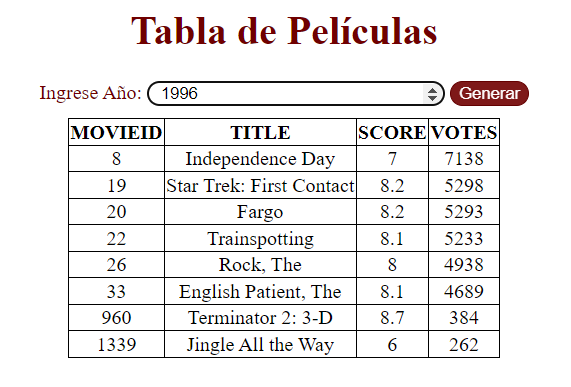
\includegraphics[width=0.7\textwidth, keepaspectratio]{img/existe.png}
      \caption{Ejecución 1}
    \end{figure}
    \item En caso de que no haya películas en la base de datos:
    \begin{figure}[H]
      \centering
      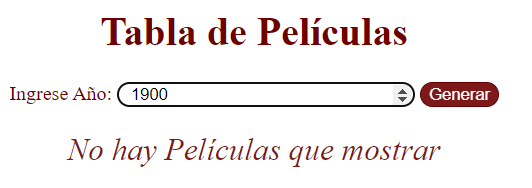
\includegraphics[width=0.7\textwidth, keepaspectratio]{img/noexiste.png}
      \caption{Ejecución 2}
    \end{figure}
  \end{itemize}
  \newpage

%%%%%%%%%%%%%%%%%%%%
	
  \subsection{Uso de GitHub}
  
%%%%%%%%%%%%%%%%%%%%

	\subsubsection{Usuario de GitHub}
  \begin{figure}[H]
    \centering
    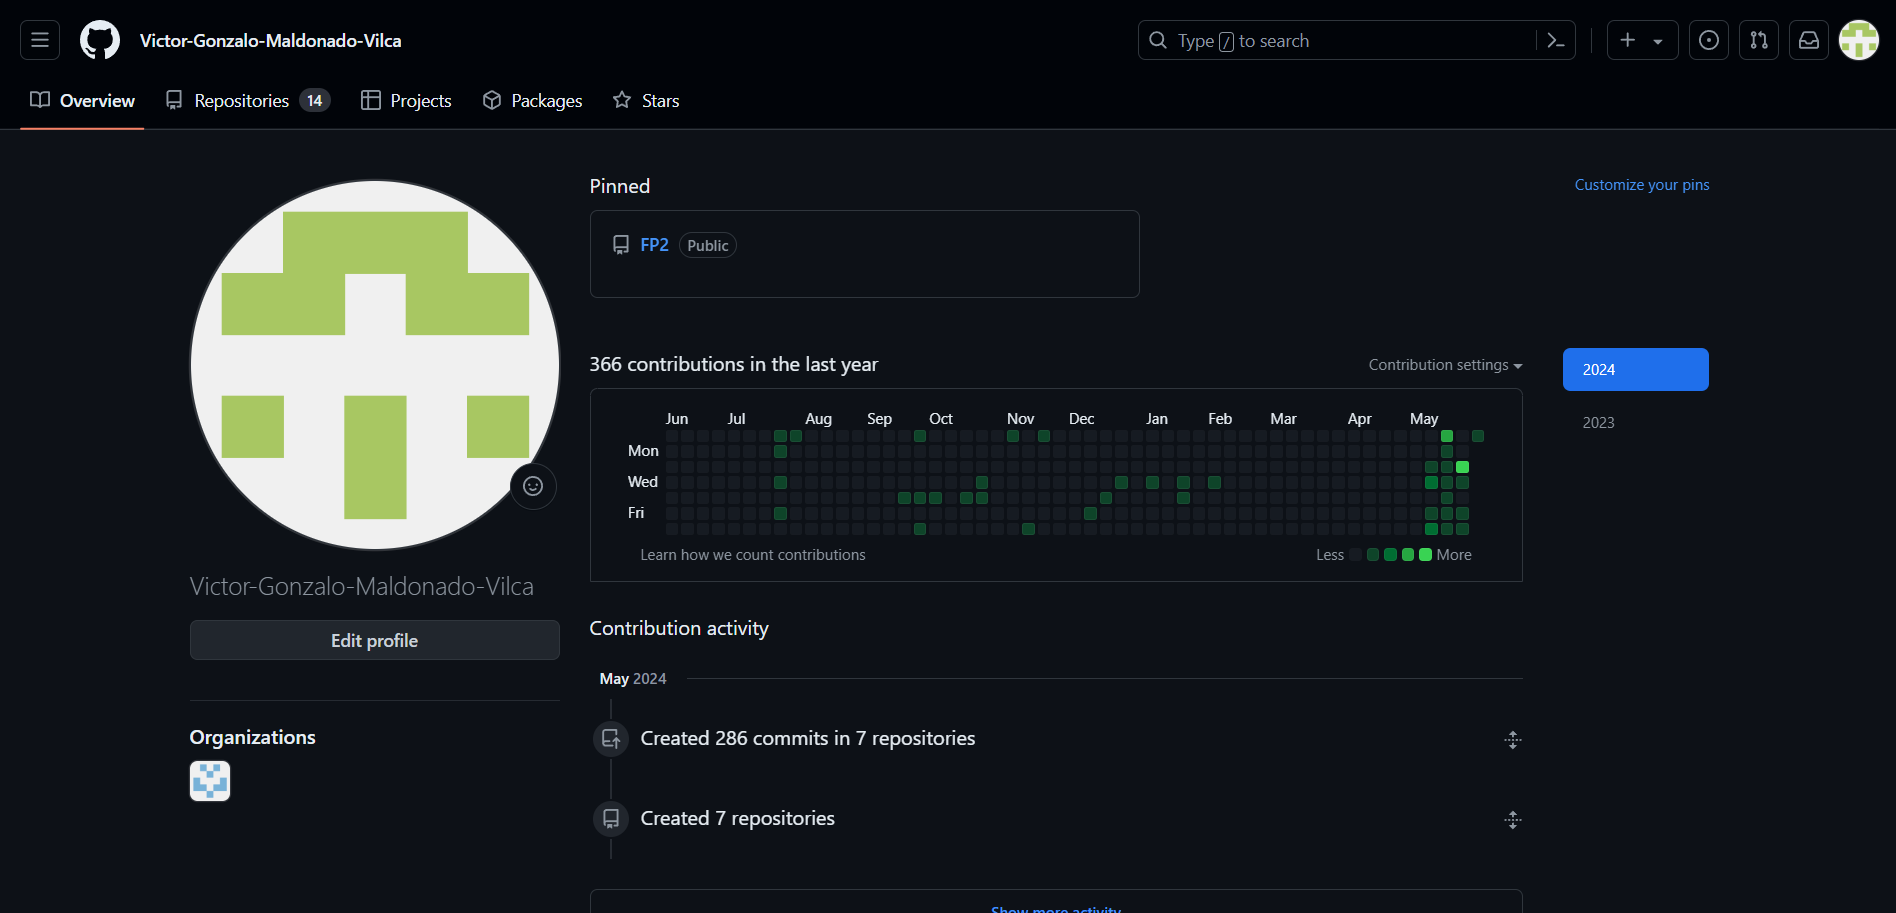
\includegraphics[width=1\textwidth, keepaspectratio]{img/usuario.png}
    \caption{Usuario GitHub}
  \end{figure}
  
%%%%%%%%%%%%%%%%%%%%

  \subsubsection{Creación de un Nuevo Repositorio}
  \begin{figure}[H]
    \centering
    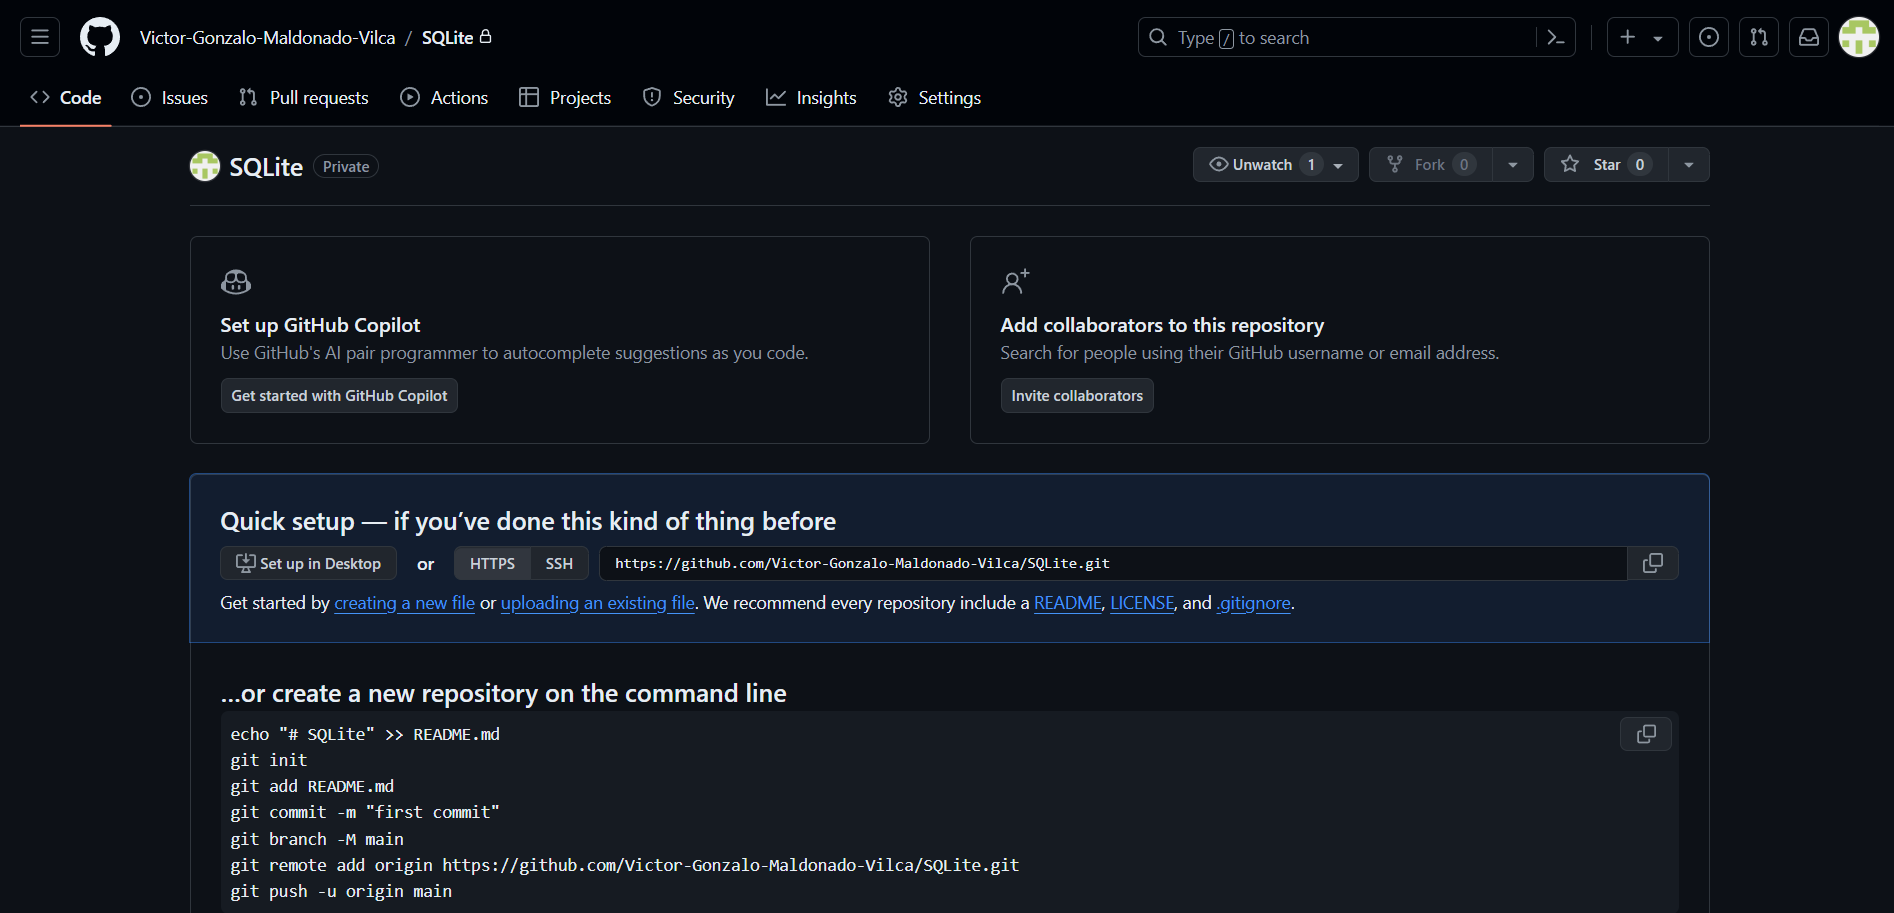
\includegraphics[width=1\textwidth, keepaspectratio]{img/crearRepo.png}
    \caption{Nuevo Repositorio SQLite}
  \end{figure}
  
%%%%%%%%%%%%%%%%%%%%  
	
  \newpage
  \subsubsection{Comandos de Configuración}
  \begin{lstlisting}[language=,caption=Configuración Inicial]
    echo "# SQLite" >> README.md
    git init
    git add README.md
    git commit -m "first commit"
    git branch -M master
    git remote add origin https://github.com/Victor-Gonzalo-Maldonado-Vilca/SQLite.git
    git push -u origin master
  \end{lstlisting}
  
%%%%%%%%%%%%%%%%%%%%  
  
  \subsubsection{Implementación de Readme.md}
  \begin{figure}[H]
    \centering
    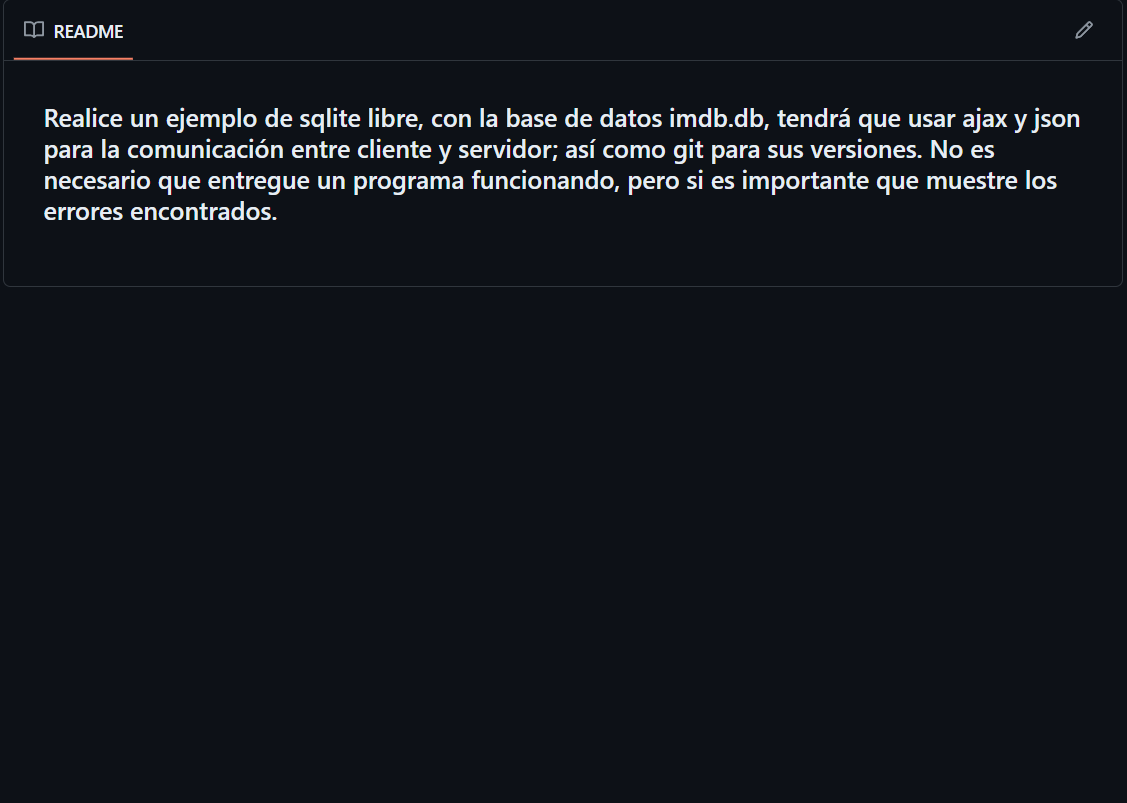
\includegraphics[width=1\textwidth, keepaspectratio]{img/Readme.png}
    \caption{Readme.md}
  \end{figure}
  \newpage
  
%%%%%%%%%%%%%%%%%%%%

	\subsubsection{Registro de cambios en mi código}
  \begin{figure}[H]
    \centering
    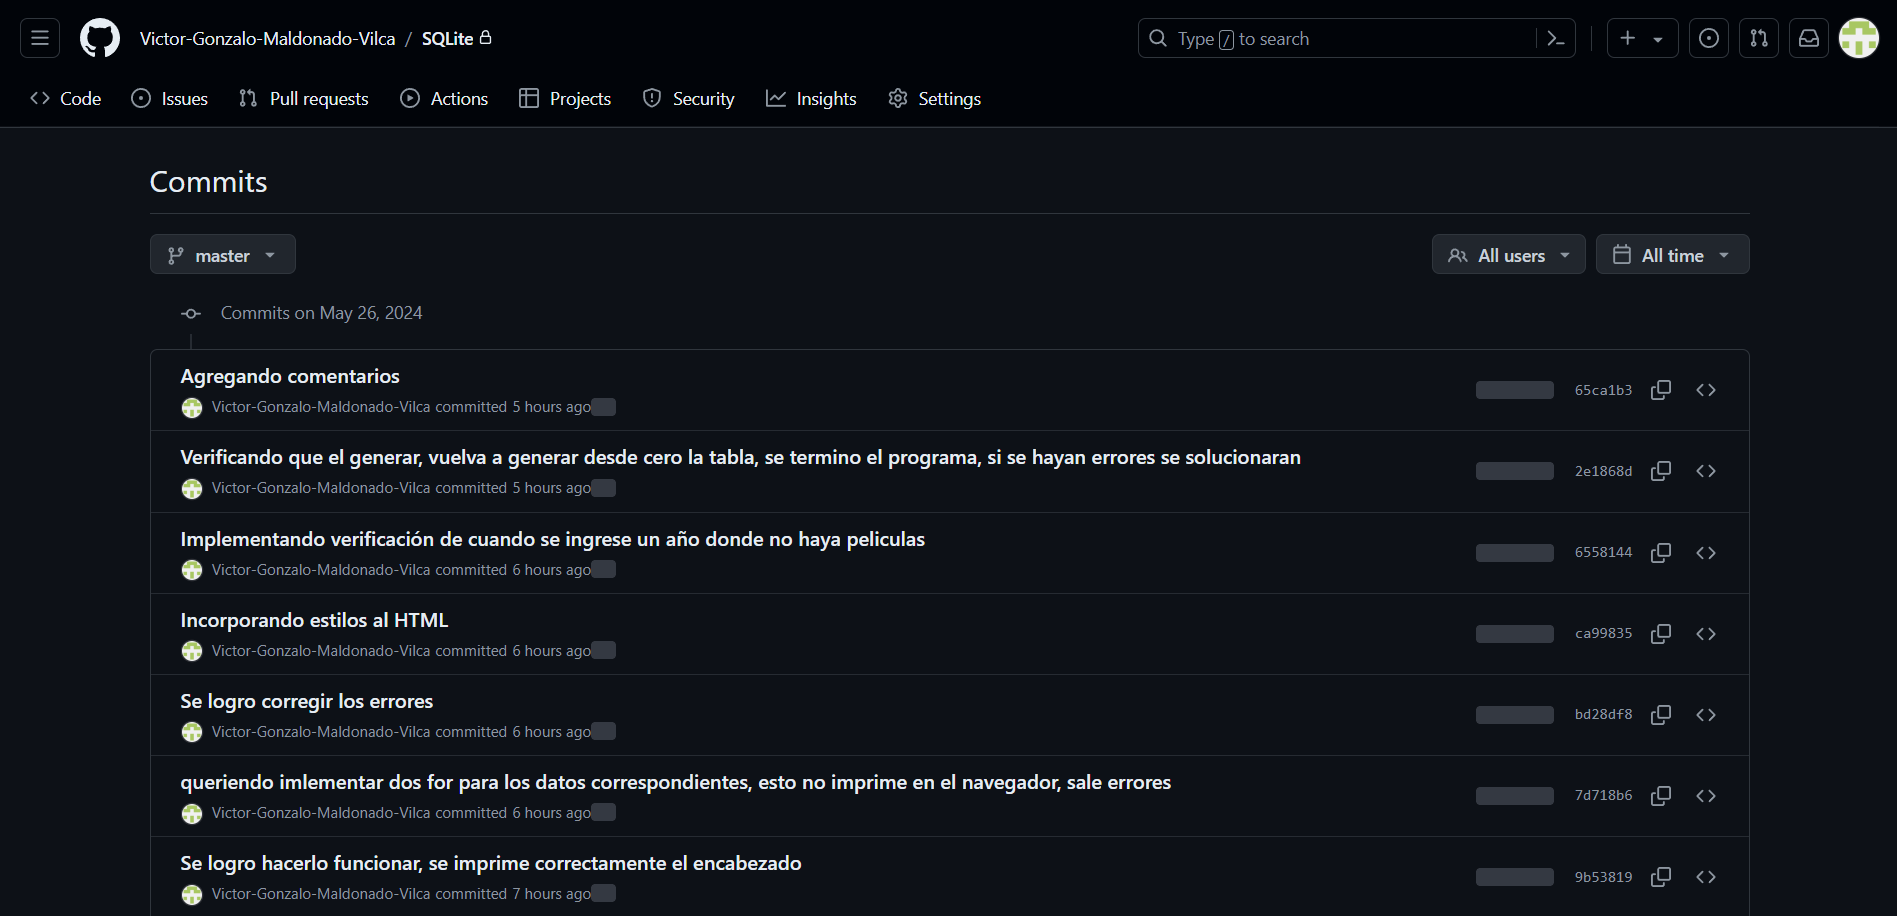
\includegraphics[width=1\textwidth, keepaspectratio]{img/commits.png}
    \caption{Commits}
  \end{figure}
	
%%%%%%%%%%%%%%%%%%%%

	\subsubsection{Repositorio}
  \begin{figure}[H]
    \centering
    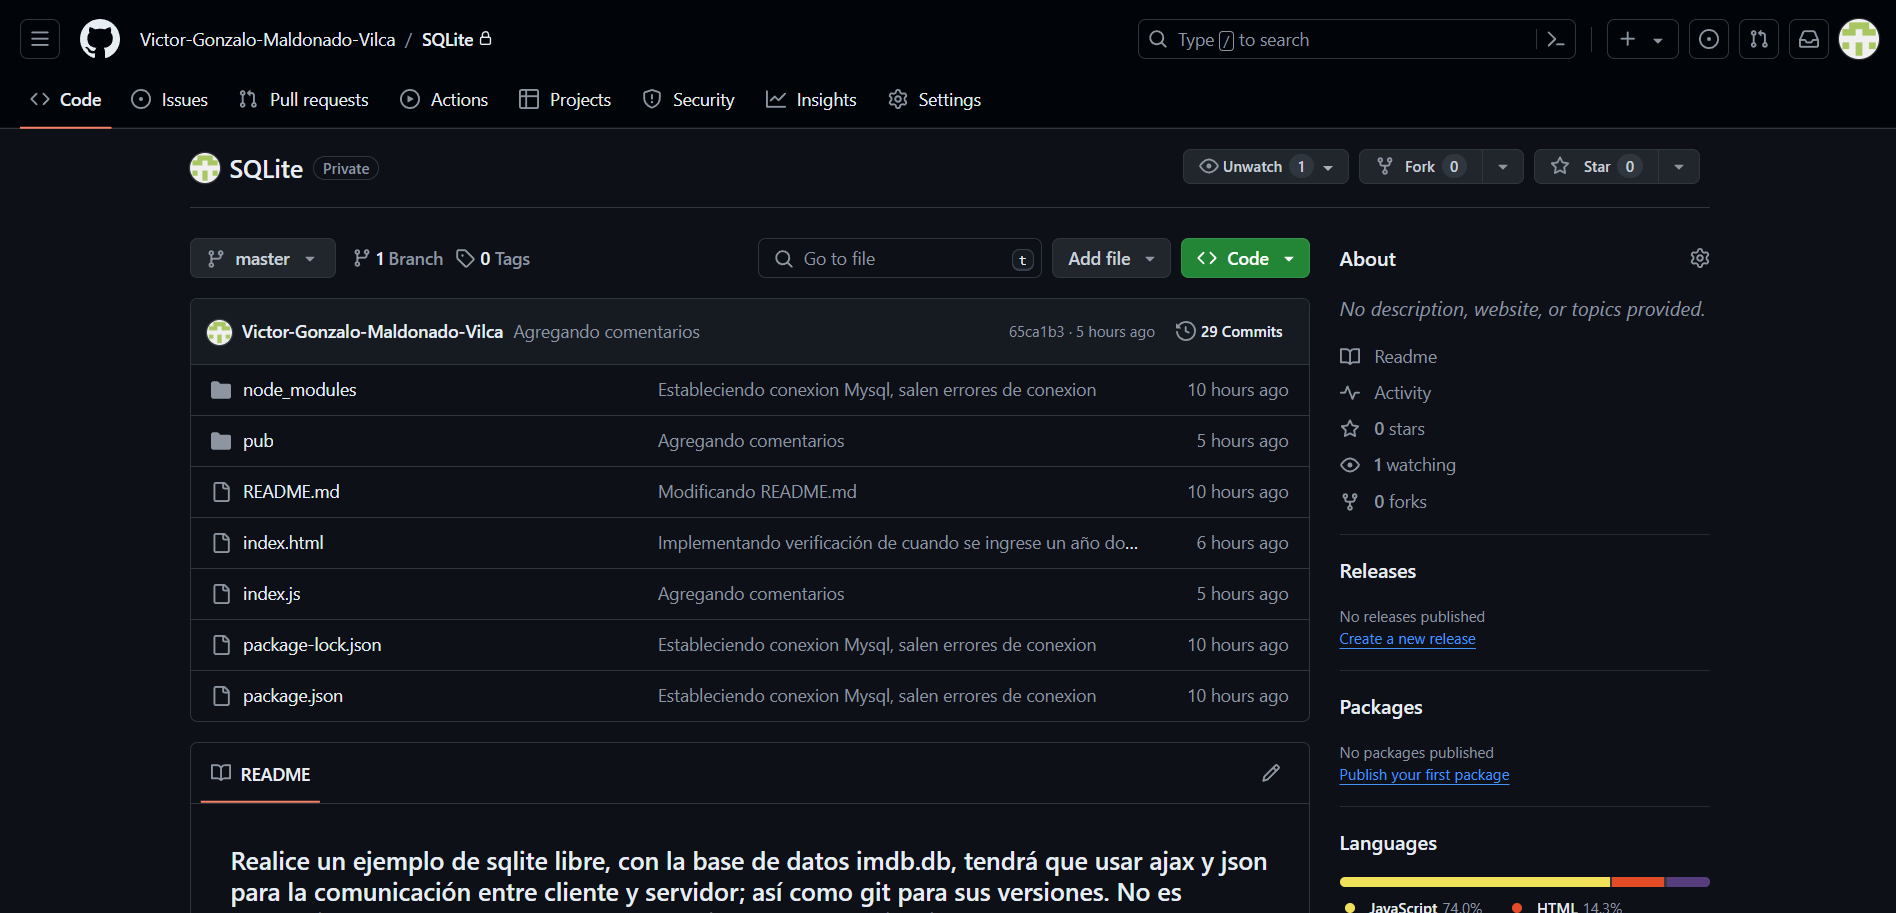
\includegraphics[width=1\textwidth, keepaspectratio]{img/repositorio.png}
    \caption{Repositorio SQLite}
  \end{figure}
  \newpage
  
%%%%%%%%%%%%%%%%%%%%

	\subsubsection{Proyecto compartido con el profesor de github}
  \begin{figure}[H]
    \centering
    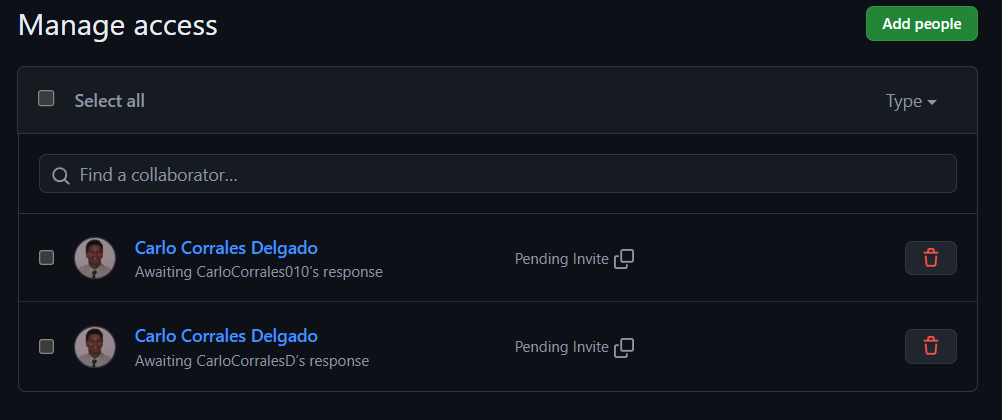
\includegraphics[width=1\textwidth, keepaspectratio]{img/Compartir.png}
    \caption{Compartir con el Docente}
  \end{figure}
  
%%%%%%%%%%%%%%%%%%%%

  \section{Recomensaciones}
  \begin{itemize}
    \item Implementar un manejo adecuado de errores al procesar datos JSON en tu servidor. Esto incluye la detección y 
      manejo de errores de análisis JSON incorrecto, así como la gestión de excepciones en tu lógica relacionada 
      con los datos JSON.
    \item Implementar un manejo adecuado de errores en tus solicitudes AJAX para informar al usuario sobre 
      posibles problemas de conexión o errores en el servidor.
    \item Fomentar las mejores prácticas de colaboración, como hacer commits atómicos y descriptivos para nuevas 
      características o correcciones de errores.
  \end{itemize}

%%%%%%%%%%%%%%%%%%%%

  \section{Conclusiones}
  \begin{itemize}
    \item Node.js es una excelente opción para desarrollar servidores debido a su naturaleza asíncrona y su capacidad 
      para manejar grandes cantidades de conexiones concurrentes de manera eficiente.
    \item AJAX facilita la comunicación entre el cliente y el servidor, lo que permite a las aplicaciones web enviar 
      y recibir datos de forma rápida y eficiente sin necesidad de recargar la página.
    \item JSON es un formato de datos simple y legible que facilita el intercambio de datos entre servidores y clientes.
    \item JSON y AJAX son tecnologías fundamentales en el desarrollo de aplicaciones web modernas, 
      mientras que Git es una herramienta esencial para la gestión del código fuente y la colaboración en proyectos de software
  \end{itemize}

%%%%%%%%%%%%%%%%%%%%
	\newpage
	\subsection{\textcolor{red}{Rúbrica para el contenido del Informe y demostración}}
	\begin{itemize}			
		\item El alumno debe marcar o dejar en blanco en celdas de la columna \textbf{Checklist} si cumplio con el ítem correspondiente.
		\item Si un alumno supera la fecha de entrega,  su calificación será sobre la nota mínima aprobada, siempre y cuando cumpla con todos lo items.
		\item El alumno debe autocalificarse en la columna \textbf{Estudiante} de acuerdo a la siguiente tabla:
	
		\begin{table}[ht]
			\caption{Niveles de desempeño}
			\begin{center}
			\begin{tabular}{ccccc}
    			\hline
    			 & \multicolumn{4}{c}{Nivel}\\
    			\cline{1-5}
    			\textbf{Puntos} & Insatisfactorio 25\%& En Proceso 50\% & Satisfactorio 75\% & Sobresaliente 100\%\\
    			\textbf{2.0}&0.5&1.0&1.5&2.0\\
    			\textbf{4.0}&1.0&2.0&3.0&4.0\\
    		\hline
			\end{tabular}
		\end{center}
	\end{table}	
	

	\end{itemize}

 
	
	\begin{table}[H]
		\caption{Rúbrica para contenido del Informe y demostración}
		\setlength{\tabcolsep}{0.5em} % for the horizontal padding
		{\renewcommand{\arraystretch}{1.5}% for the vertical padding
		%\begin{center}
		\begin{tabular}{|p{2.7cm}|p{7cm}|x{1.3cm}|p{1.2cm}|p{1.5cm}|p{1.1cm}|}
			\hline
    		\multicolumn{2}{|c|}{Contenido y demostración} & Puntos & Checklist & Estudiante & Profesor\\
			\hline
			\textbf{1. GitHub} & Hay enlace URL activo del directorio para el  laboratorio hacia su repositorio GitHub con código fuente terminado y fácil de revisar. &2 &X &2 & \\ 
			\hline
			\textbf{2. Commits} &  Hay capturas de pantalla de los commits más importantes con sus explicaciones detalladas. (El profesor puede preguntar para refrendar calificación). &4 &X &4 & \\ 
			\hline 
			\textbf{3. Código fuente} &  Hay porciones de código fuente importantes con numeración y explicaciones detalladas de sus funciones. &2 &X &2 & \\ 
			\hline 
			\textbf{4. Ejecución} & Se incluyen ejecuciones/pruebas del código fuente  explicadas gradualmente. &2 &X &2 & \\ 
			\hline			
			\textbf{5. Pregunta} & Se responde con completitud a la pregunta formulada en la tarea.  (El profesor puede preguntar para refrendar calificación).  &2 &X &2 & \\ 
			\hline	
			\textbf{6. Fechas} & Las fechas de modificación del código fuente estan dentro de los plazos de fecha de entrega establecidos. &2 &X &2 & \\ 
			\hline 
			\textbf{7. Ortografía} & El documento no muestra errores ortográficos. &2 &X &2 & \\ 
			\hline 
			\textbf{8. Madurez} & El Informe muestra de manera general una evolución de la madurez del código fuente,  explicaciones puntuales pero precisas y un acabado impecable.   (El profesor puede preguntar para refrendar calificación).  &4 &X &4 & \\ 
			\hline
			\multicolumn{2}{|c|}{\textbf{Total}} &20 & &20 & \\ 
			\hline
		\end{tabular}
		%\end{center}
		%\label{tab:multicol}
		}
	\end{table}


%%%%%%%%%%%%%%%%%%%%%%%%%%%%%%%%%%%%%%%%%%%%%%%%%%%%%%%%%%%%%%%%%%%
	
  \newpage
  \section{Referencias}
  \begin{itemize}
    \item \url{https://nodejs.org/en}
    \item \url{https://www.apachefriends.org/es/index.html}
    \item \url{https://www.w3schools.com/}
  \end{itemize}

%%%%%%%%%%%%%%%%%%%% 
%\clearpage
%\bibliographystyle{apalike}
%\bibliographystyle{IEEEtranN}
%\bibliography{bibliography}
			
\end{document}
